\chapter{The Run-3 Operations of the CMS detector}
\label{chap:Ops}

The \ac{CMS} detector resumed data-taking in July 2022, following the start of the Run-3 of the \ac{LHC}. When compared to the Run-2, the center of mass energy of the proton beams increase from 13 TeV to 13.6 TeV in Run 3. At the same time, the peak instantaneous luminosity is kept at the same or higher level as the 2018 data-taking year ($2\times10^{34}~\textsf{cm}^{-2}\textsf{s}^{-1}$), as illustrated in Figure~\ref{fig:peak}.

\begin{figure}[tbh!]
 \begin{center}
 \begin{tabular}{c}
 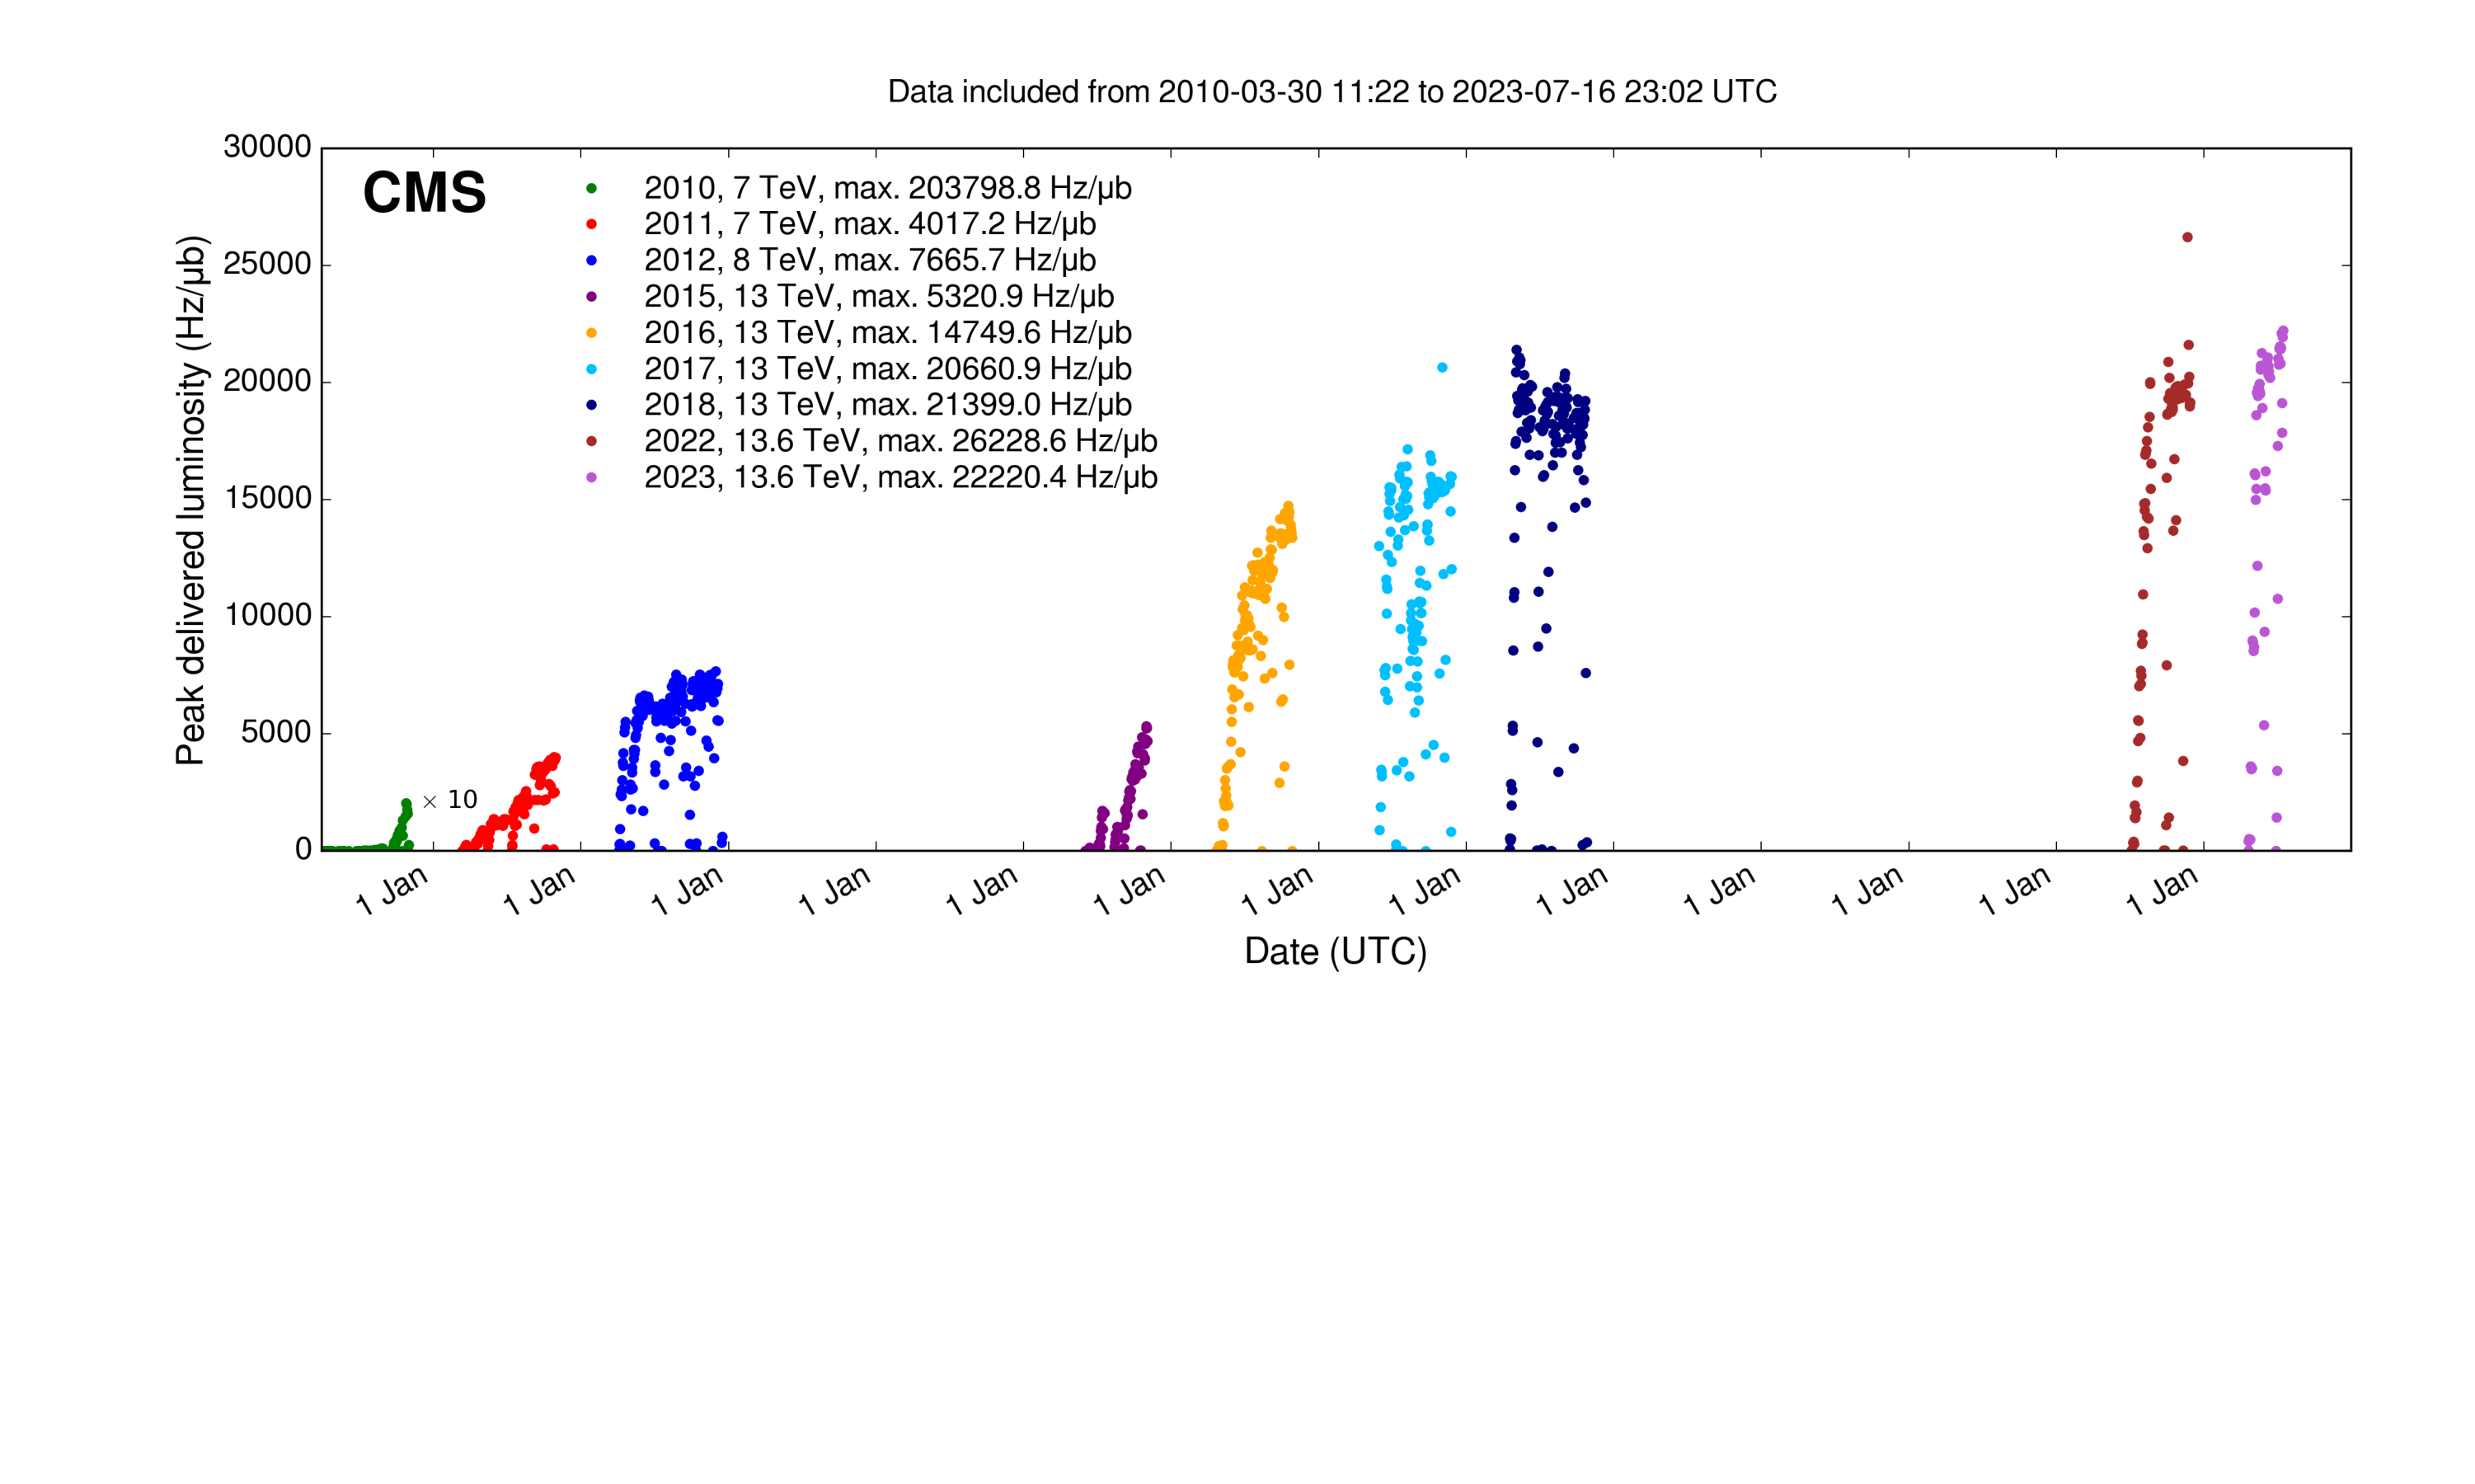
\includegraphics[width=\textwidth]{figures/Part2/Operation/peak_lumi_pp}
 \end{tabular}
 \caption{Peak luminosity versus day delivered to \ac{CMS} during stable beams and for proton-proton collisions, adapted from~\cite{twiki:lumi}.}
 \label{fig:peak}
 \end{center}
\end{figure}

Operations of the \ac{CMS} detector is coordinated by the \ac{CMS} Run Coordination, which is introduced in \autoref{sec:RC}. The \ac{CMS} control room is the commanding center of the \ac{CMS} operations, which is staffed 24$\times$7 during active data-taking period. Personnel who monitor and operate the \ac{CMS} detector from the control room are referred to as the ``central shift crew``, which is discussed further in \autoref{sec:ControlRoom}. In the In the context of detector operations, the principle contacts of the subsystems of the \ac{CMS} detector are known as the \ac{DOC} experts, or simply the \acp{DOC}. Core duties of one of the \acp{DOC}, the tracker \ac{DOC}, are described in \autoref{sec:DOC}.

\section{The CMS Run Coordination}
\label{sec:RC}

The \ac{CMS} Run Coordination is nominally headed by two Run Coordinators and one deputy Run Coordinator whose mandate is to ensure the successful running of \ac{CMS}. The Run Coordinators oversee all operations activities at the \ac{CMS} and are nominally appointed for a two-year term. The Run Coordinators work closely with the Technical Coordination, the \ac{LHC} team, and the subsystem operations teams to draft the long-term strategic goals for the central operations, as well as commissioning efforts in subsystems. These strategic goals are helped achieved by the \acp{RFM} who serve as the liaison between the Run Coordination and the central shift crew, as illustrated in Figure~\ref{fig:RC}.

\begin{figure}[tbh!]
 \begin{center}
 \begin{tabular}{c}
 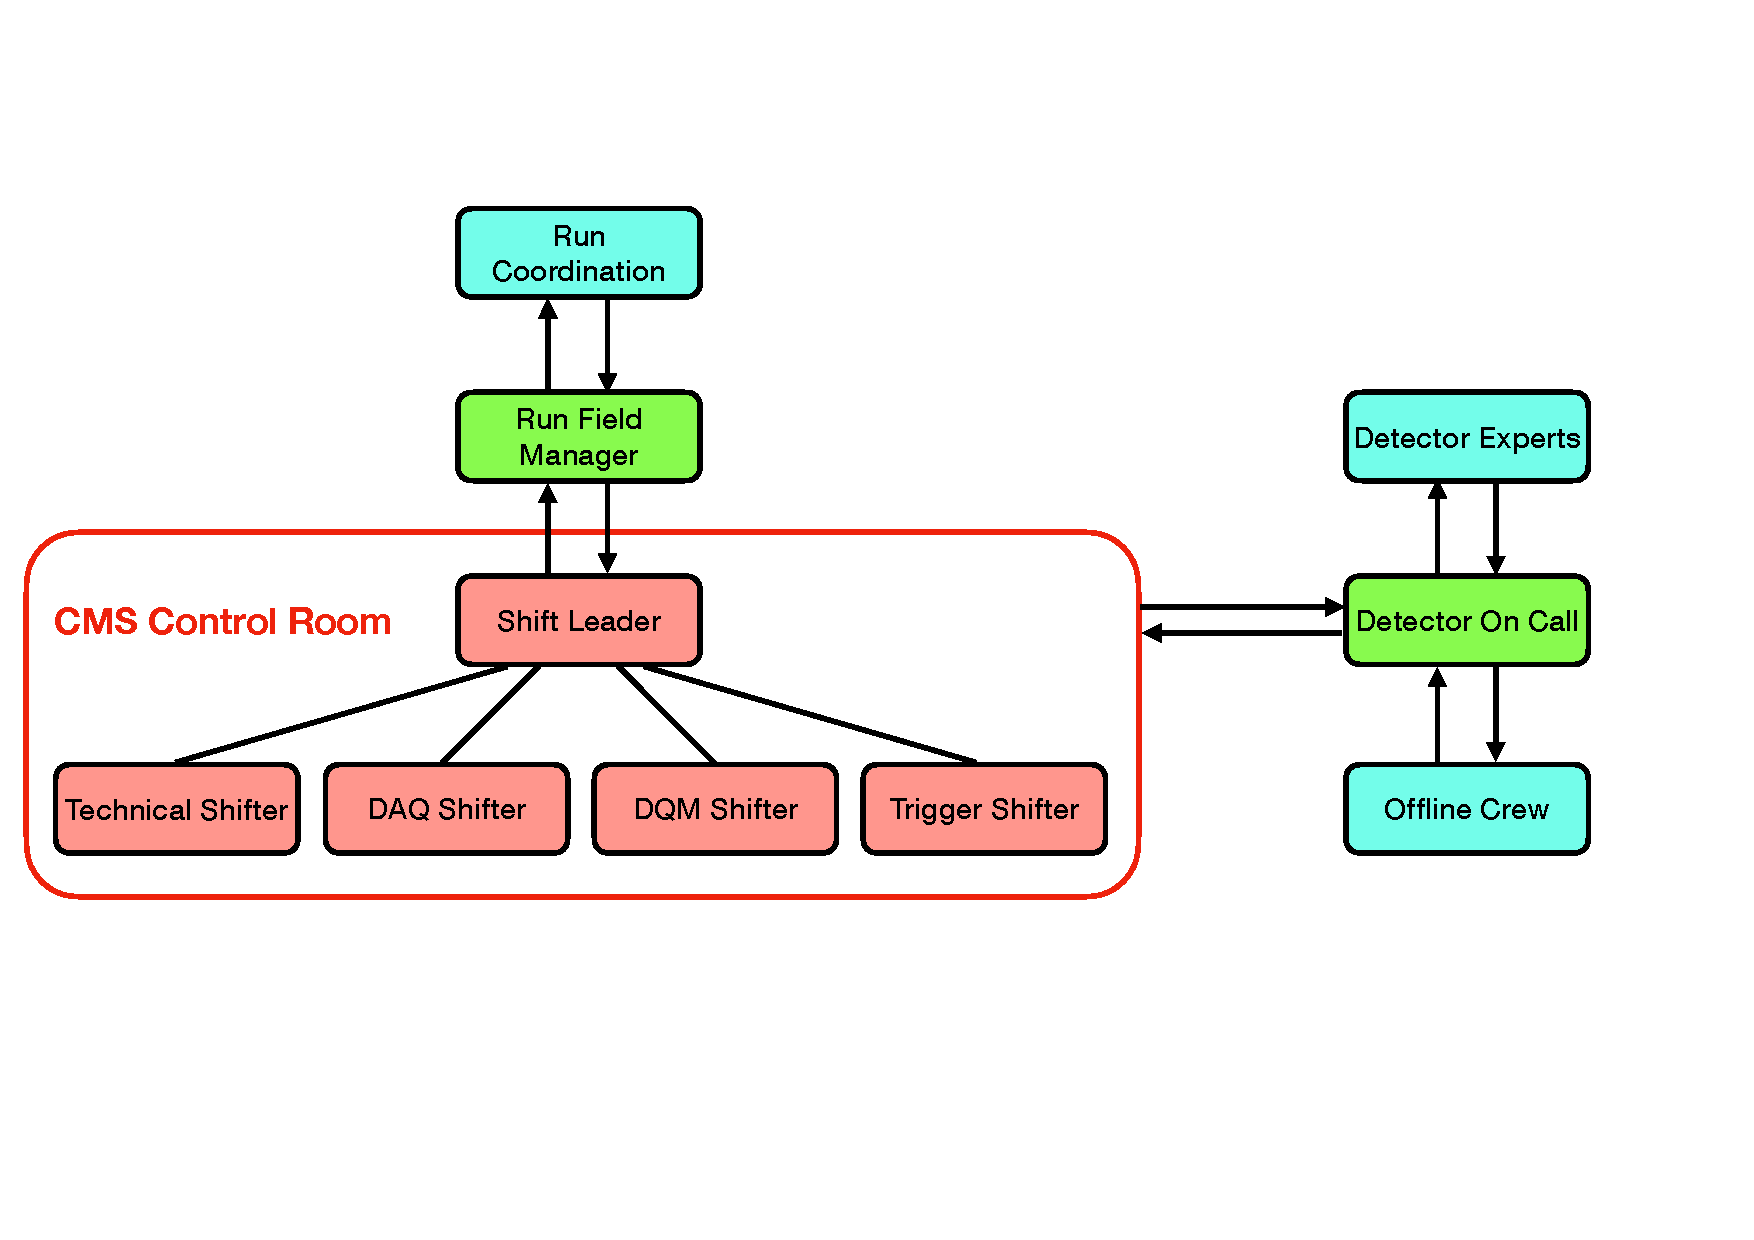
\includegraphics[width=0.9\textwidth]{figures/Part2/Operation/RC}
 \end{tabular}
 \caption{Main communication paths between various personnel within the \ac{CMS} Run organization. The \ac{SL}, technical, \ac{DAQ}, \ac{DQM}, and the trigger shifters are required to be present at the \ac{CMS} control room 24$\times$7. The \acp{RFM} and the \acp{DOC} are nominally present at the control room during the working hours. The Run Coordinators, subsystem expects, and offline shifters are not required to be at the control room although they often do.}
 \label{fig:RC}
 \end{center}
\end{figure}

The \ac{RFM} team is nominally appointed for a two-week term and typically consists of two members who have extended experiences in various roles of operations, particularly the \ac{SL}. The \acp{RFM}, together with the Run Coordinators, organize the \ac{CMS} daily run meetings in the morning on every weekday to collect the feedback \& requests from the subsystem \acp{DOC} and set the daily run plan. The \acp{RFM} also facilitate the \ac{SL} in implementing these plans as the \ac{SL}, like the rest of the central shift crew, nominally does not attend the daily run meeting.

\section{Central Shift Crew}
\label{sec:ControlRoom}

The \ac{CMS} detector is considered to be ``running'' when all high-voltage channels are switched on and taking data. During this period, operations of various subsystems of the \ac{CMS} detector are controlled by the central shift crew, which consists of five members: the \ac{SL}, technical, \ac{DAQ}, \ac{DQM}, and trigger shifters, as illustrated in Figure~\ref{fig:ControlRoom}. 

\begin{figure}[tbh!]
 \begin{center}
 \begin{tabular}{c}
 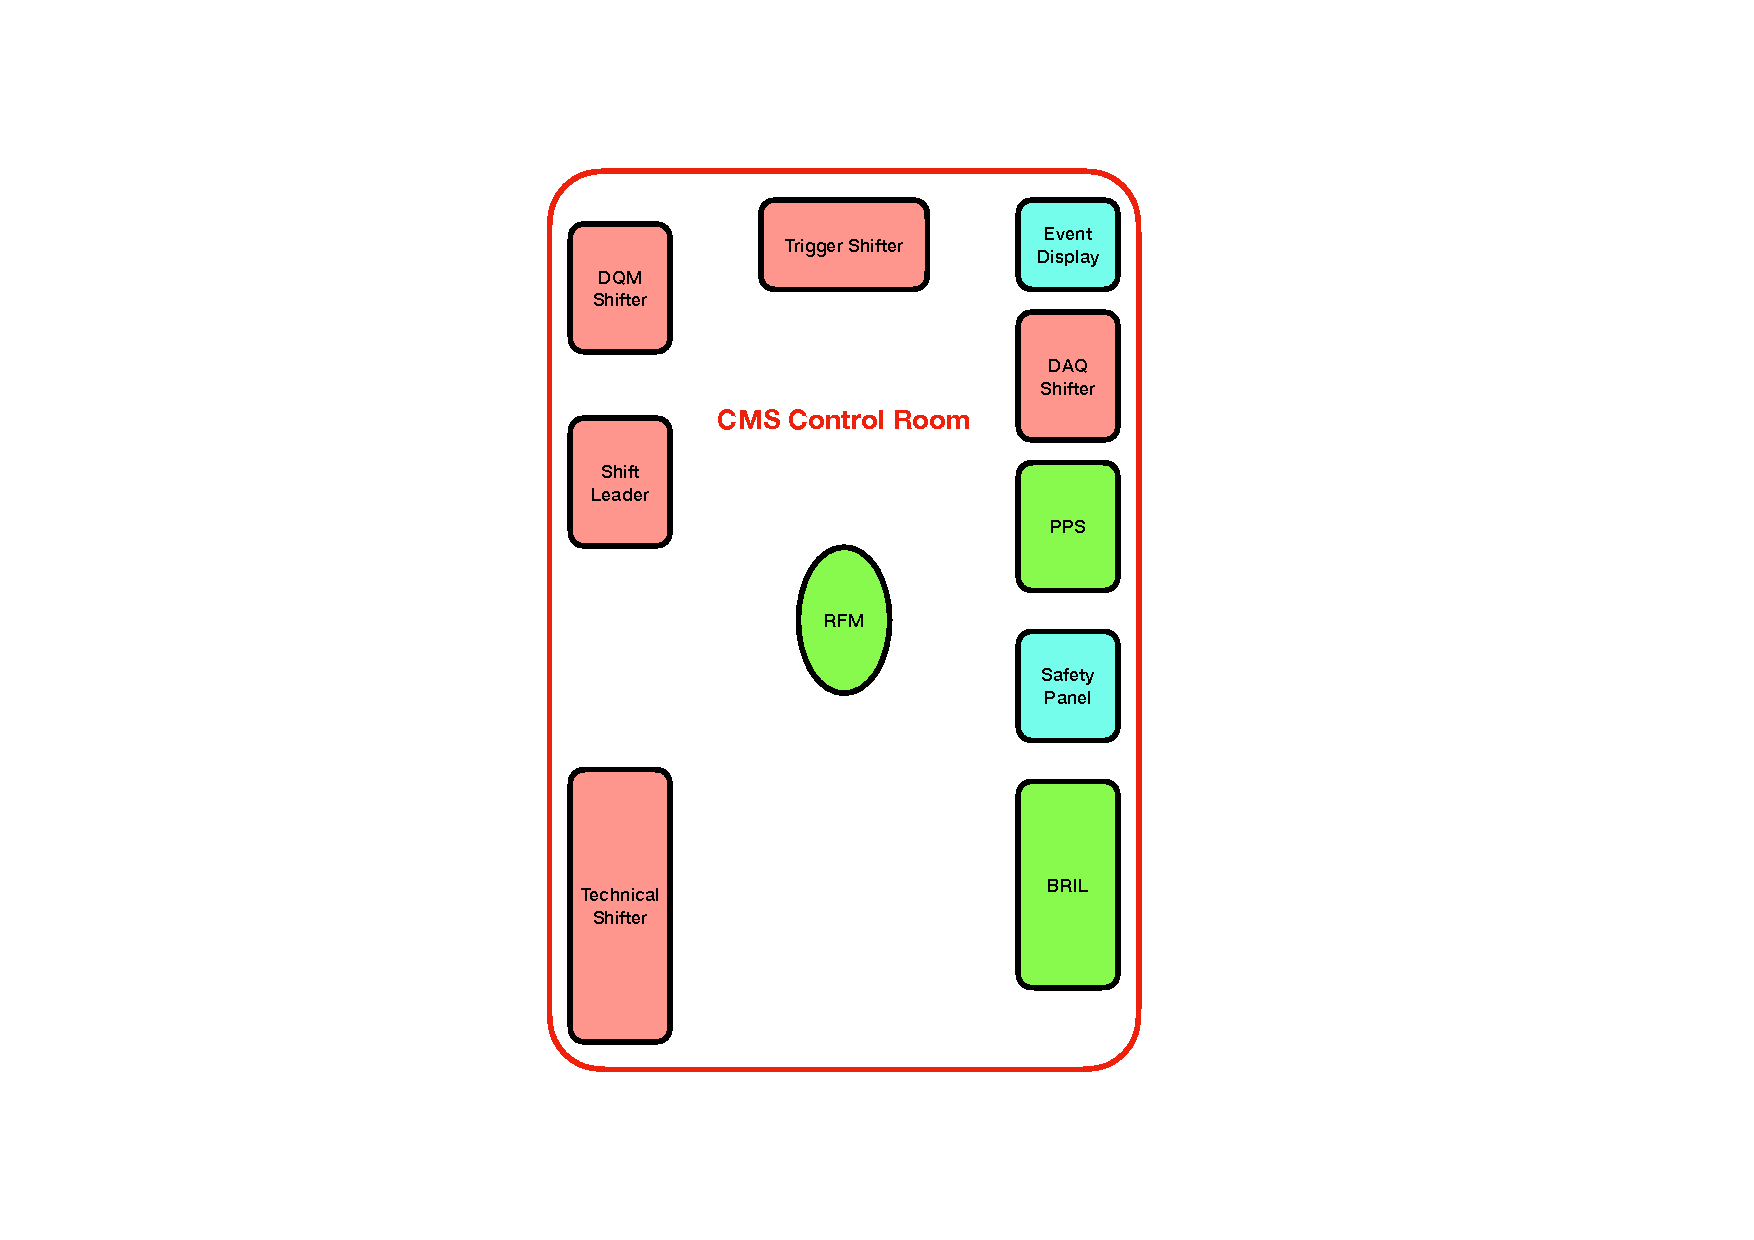
\includegraphics[width=0.4\textwidth]{figures/Part2/Operation/ControlRoom}
 \end{tabular}
 \caption{A sketch of the layout of the \ac{CMS} control room. The area where the event display and the safety panel is located is nominally not designated to any personnel. The \ac{PPS}~\cite{CMS:2014sdw} and \ac{BRIL}~\cite{CMS:2008xjf} groups have designated working space in the control room although these groups do not maintain a 24$\times$7 presence in the area.}
 \label{fig:ControlRoom}
 \end{center}
\end{figure}

In order to maximize the luminosity output and data taking efficiency, the \ac{LHC} normally takes no break at night once it starts producing high intensity collisions. The \ac{CMS} detector is therefore kept on 24$\times$7 once the \ac{LHC} is operational, and members of the \ac{CMS} Collaboration take eight hours shifts in relay from the control room. The running period when all subsystems are included in the data taking is considered to be a ``global run''. The data collected from global runs are then screened and certified by the \ac{CMS} \ac{PPD} group for physics analyses. 

The \ac{SL} is nominally considered to be the leader of the central shift crew, whose primary duty is to ensure a successful execution of the daily run plan. The \ac{SL} coordinates all activities in the \ac{CMS} control room and communicates with the \acp{RFM}, \ac{CMS} Run Coordination, as well as the \ac{CCC} about the operations. The \ac{SL} is also simultaneously the \ac{SLIMOS}, who is in charge of the safety during the operation, together with the technical shifter. 

The technical shifter is responsible for all things related to the \ac{DCS} and \ac{DSS}. The technical shifter is often the ``first responder'' when problems arise in the \ac{CMS} detector or the surrounding infrastructures during the operation. The technical shifter coordinates the responses to these problems with the \acp{DOC}, \ac{CMS} Technical Coordination, as well as \ac{CERN} technical team. The technical shifter is also co-responsible for the safety during the operation as safety duties are nominally delegated from the \ac{SL} to the technical shifter. These duties include: monitoring and responding the \ac{DSS} alerts, overseeing the underground access and the usage of all safety equipments in the control room, and performing safety tours in the surface as well as the underground area. 

The core duty of the \ac{DAQ} shifter is to ensure a smooth and efficient data taking, where the efficiency is roughly measured as the ratio of the recorded luminosity and the delivered luminosity. When a subsystem \ac{DAQ}  runs into problems it can stop a global run and block the whole system entirely from running again, resulting in the so called ``downtime'', which undermines the taking data taking efficiency. The \ac{DAQ} shifter is in communication with the \ac{SL} and \acp{DOC} about the readiness of all subsystems before initializing a global run, and is heavily involved in the troubleshooting when subsystems are uncooperative in global runs.

The \ac{DQM} shifter is responsible for the quality of the data taken by the \ac{CMS} detector. The \ac{DQM} shifter is nominally the first person to spot problems (related to data quality) in the running detector and is trained to do so by familiarizing him- or herself with the ``normal'' as well as the faulty patterns of the data collected in all subsystems. Traditionally \ac{DQM} shifters attend shifts in person from the \ac{CMS} control room just like the \ac{SL}, technical, and \ac{DAQ} shifters. In recent years, especially since the COVID-19 outbreak, more flexibility has been given to the \ac{DQM} shifters, who can now choose to work from one of the \ac{CMS} Remote Operations Centers or from home.

The \ac{L1} and \ac{HLT} rates during the data taking is monitored by the trigger shifter, who along with the \ac{SL} determines the appropriate prescale column based off the real time \ac{L1} rate. The trigger shifter makes sure all trigger subsystems are running correctly and is in communication with the \ac{L1} and \ac{HLT} \acp{DOC} when a troubleshooting is needed. Similar to \ac{DQM} shifters, trigger shifters have the option to work remotely provided that they have done in person shifts more than a few times and are sufficiently familiar with the procedure. 

\section{Tracker Detector On-call Expert}
\label{sec:DOC}

Subsystems like the tracker do not maintain a 24$\times$7 presence at the \ac{CMS} control room. Instead, their shifters, known as \acp{DOC}, are appointed for one week and nominally only join the central shift crew in the control room during working hours. After the working hours, \acp{DOC} remain accessible by phone and they are ready to go the control room at anytime should the situation require. 

The term ``tracker \ac{DOC}'' usually refers to the strip tracker \ac{DOC} while the pixel tracker has its own \ac{DOC} known as the ``pixel \ac{DOC}''. The tracker \ac{DOC} is the main point of contact for the strip tracker during his or her mandate, which typically lasts for one week. On behalf of the strip tracker operations team, the tracker \ac{DOC} reports the status of the strip tracker at the \ac{CMS} daily run meeting. He or she also monitors the state of the strip tracker in all aspects (e.g. power, \ac{DAQ}) and coordinates the daily activities with tracker detector experts and the tracker offline shift crew whose primary duty is the certification of the data collected by tracker. 

A stable and safe operation of the strip tracker requires both well-trained tracker \acp{DOC} as well as a modern \ac{DCS}. Built on top of the industrial product “WinCC”, the \ac{CMS} \ac{TCS}~\cite{Shah:2009zz,Karimeh:2020tzx} is designed to monitor the environmental conditions and safely operate the detector. As part of the \ac{TCS} software, a \ac{FSM} toolkit is introduced. It is a powerful tool that assists operators in their daily job. It groups the power, cooling, dry gas and monitoring systems defined in the four \ac{TCS} projects in one hierarchical tree. The global state of the detector is continuously evaluated and made visible from the root Tracker \ac{FSM} node giving critical information to the detector operator, as illustrated in Figure~\ref{fig:DCS}.

\begin{figure}[tbh!]
 \begin{center}
 \begin{tabular}{c}
 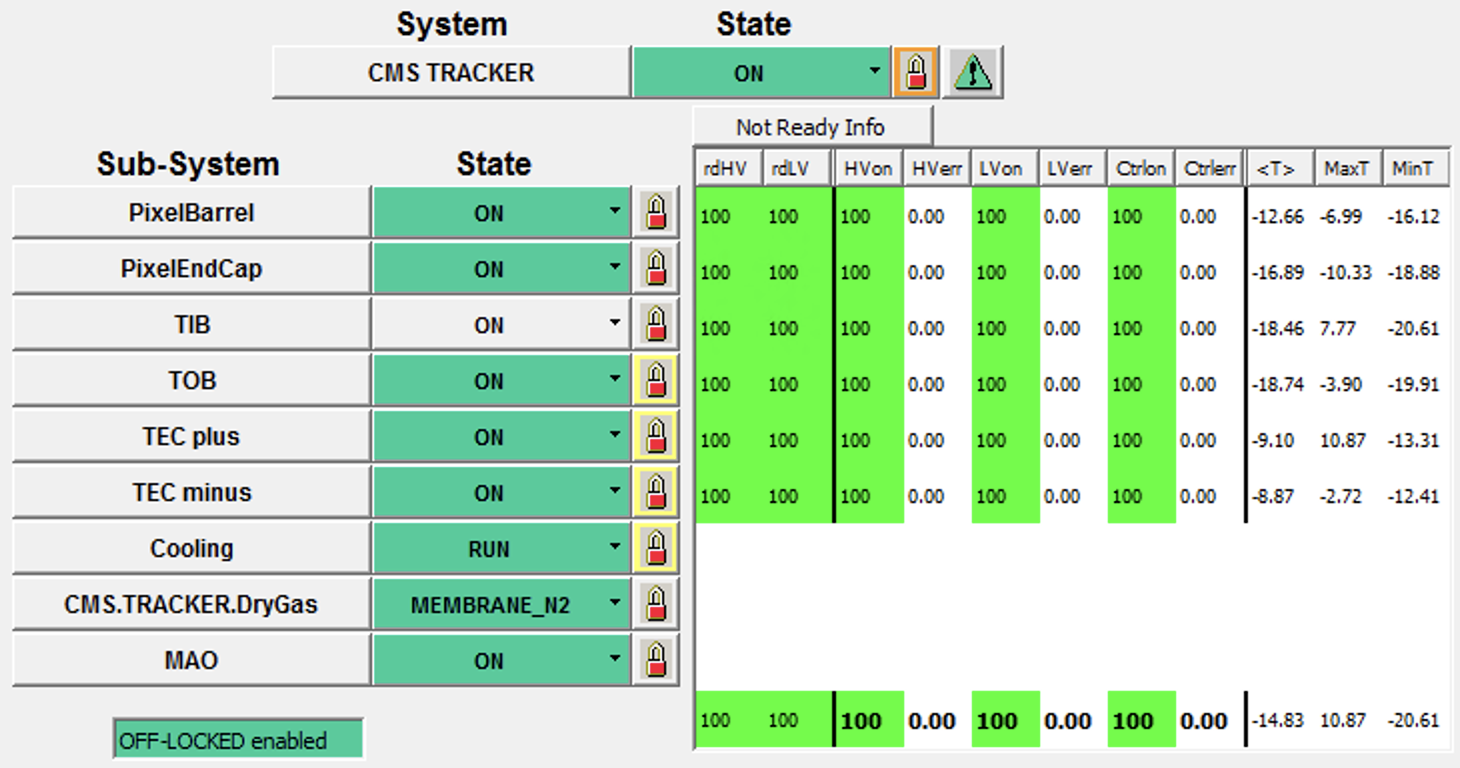
\includegraphics[width=0.8\textwidth]{figures/Part2/Operation/TrackerDCS}
 \end{tabular}
 \caption{Main panel of the tracker \ac{FSM}, screenshotted in October 2022 during the Run-3 data taking.}
 \label{fig:DCS}
 \end{center}
\end{figure}